%%%%%%%%%%%%%%%%%%%%%%%%%%%%%%%%%%%%%%%%%%%%%%%%%%%%%%%%%%%%%%%%%%%%%%%%%%%%%%%%%%%%%%%%%%%%%%%%%%%%%%%%%%%%%%%%%%%%%%%%%%%%%%%%%%%%%%%%%%%%%%%%%%%%%%%%%%%
% This is just an example/guide for you to refer to when submitting manuscripts to Frontiers, it is not mandatory to use Frontiers .cls files nor frontiers.tex  %
% This will only generate the Manuscript, the final article will be typeset by Frontiers after acceptance.   
%                                              %
%                                                                                                                                                         %
% When submitting your files, remember to upload this *tex file, the pdf generated with it, the *bib file (if bibliography is not within the *tex) and all the figures.
%%%%%%%%%%%%%%%%%%%%%%%%%%%%%%%%%%%%%%%%%%%%%%%%%%%%%%%%%%%%%%%%%%%%%%%%%%%%%%%%%%%%%%%%%%%%%%%%%%%%%%%%%%%%%%%%%%%%%%%%%%%%%%%%%%%%%%%%%%%%%%%%%%%%%%%%%%%

%%% Version 3.4 Generated 2018/06/15 %%%
%%% You will need to have the following packages installed: datetime, fmtcount, etoolbox, fcprefix, which are normally inlcuded in WinEdt. %%%
%%% In http://www.ctan.org/ you can find the packages and how to install them, if necessary. %%%
%%%  NB logo1.jpg is required in the path in order to correctly compile front page header %%%

\documentclass[utf8]{frontiersSCNS} % for Science, Engineering and Humanities and Social Sciences articles
%\documentclass[utf8]{frontiersHLTH} % for Health articles
%\documentclass[utf8]{frontiersFPHY} % for Physics and Applied Mathematics and Statistics articles

%\setcitestyle{square} % for Physics and Applied Mathematics and Statistics articles
\usepackage{url,hyperref,lineno,microtype,subcaption}
\usepackage[onehalfspacing]{setspace}
\usepackage{float}
\usepackage{gensymb}

\usepackage[compact]{titlesec}
\titlespacing{\section}{0pt}{2ex}{1ex}
\titlespacing{\subsection}{0pt}{1ex}{0ex}
\titlespacing{\subsubsection}{0pt}{0.5ex}{0ex}

\usepackage{enumitem}


\linenumbers


% Leave a blank line between paragraphs instead of using \\


\def\keyFont{\fontsize{8}{11}\helveticabold }
\def\firstAuthorLast{Sample {et~al.}} %use et al only if is more than 1 author
\def\Authors{Xinyu Yao\,$^{1}$ and Selvyn Perez\,$^{1}$}
% Affiliations should be keyed to the author's name with superscript numbers and be listed as follows: Laboratory, Institute, Department, Organization, City, State abbreviation (USA, Canada, Australia), and Country (without detailed address information such as city zip codes or street names).
% If one of the authors has a change of address, list the new address below the correspondence details using a superscript symbol and use the same symbol to indicate the author in the author list.
\def\Address{$^{1}$Data Science, Columbian College of Arts and Science, George Washington University, Washington, DC, USA \\
}
% The Corresponding Author should be marked with an asterisk
% Provide the exact contact address (this time including street name and city zip code) and email of the corresponding author
\def\corrAuthor{Xinyu Yao}
\def\corrEmail{xinyu\textunderscore yao@gwu.edu}

\begin{document}
\onecolumn
\firstpage{1}

\title[Running Title]{Wheat Head Detection from High Resolution RGB Images Using Convolutional Neural Network} 

\author[\firstAuthorLast ]{\Authors} %This field will be automatically populated
\address{} %This field will be automatically populated
\correspondance{} %This field will be automatically populated

\extraAuth{}% If there are more than 1 corresponding author, comment this line and uncomment the next one.
%\extraAuth{corresponding Author2 \\ Laboratory X2, Institute X2, Department X2, Organization X2, Street X2, City X2 , State XX2 (only USA, Canada and Australia), Zip Code2, X2 Country X2, email2@uni2.edu}


\maketitle
\begin{abstract} Wheat head density estimation is an appealing trait for plant breeders. Current manual counting is tedious and inefficient. In this study three types of CNN architectures were investigated: (i) YOLO, (ii) EfficientDet, and (iii) Faster R-CNN. Models were evaluated on the mean average precision at different intersections over union (IoU) thresholds, ranging from 0.5 to 0.75 with a step size of 0.05. Further, the number of wheat heads detected from the RGB images will be compared with the number of wheat heads labelled. YOLO got the best performance with AP$_{.5...0.75}$  of 0.75, mAP@0.5 of 0.86, and rMSE of 10\%.
\tiny
 \keyFont{ \section{Keywords:} Wheat head; Object detection; Object counting; Field imaging; Convolutional neural networks} %All article types: you may provide up to 8 keywords; at least 5 are mandatory.
\end{abstract}

\section{Introduction} 
\par
Wheat head density is associated with crop yield, but is a difficult and tedious trait for breeders to efficiently measure. Further, it is prone to sampling errors when the sampling area is small due to limited human resources. Computer vision approaches provide a potential solution to increase the throughput as well as the spatial representativeness, leading potentially to an improved accuracy. A number of studies based on high spatial resolution imaging systems applied to plant phenotyping under field conditions have received much attention in recent years \citep{li2014review}.
\par
While previous studies \citep{milioto2018real, ubbens2018use, madec2019ear} have tested wheat head detection methods on individual datasets, in practice these deep learning models are difficult to scale to real-life phenotyping platforms, since they are trained on limited datasets, with expected difficulties when extrapolating to new situations. Most training datasets are limited in terms of genotypes, geographic areas and observational conditions. Wheat head morphology may significantly differ between genotypes with notable variation in head morphology, including size, inclination, color and the presence of awns \citep{david2020global}. The appearance of heads and the background canopy also change significantly from emergence to maturation due to ripening and senescence \citep{anderegg2020spectral}. Further, planting densities and patterns vary globally across different cropping systems and environments, with possible overlap between heads for the higher head densities \citep{david2020global}. To fill the need for a large and diverse wheat head dataset with consistent labelling, the Global Wheat Head Detection (GWHD) dataset \citep{david2020global} was published, which can be used to benchmark methods proposed in the computer vision community. The GWHD dataset results from the harmonization of several datasets coming from seven countries and three continents, at different growth stages with a wide range of genotypes.
\par
The advances in computation capacity along with the availability of very large collections of labelled images have fostered enhanced machine learning methods based on convolutional neural networks (CNNs) in the field of computer vision \citep{lecun2015deep}. Existing object detectors are mostly categorized by whether they have a region-of interest proposal step (two-stage) \citep{girshick2014rich, ren2015faster} or not (one-stage) \citep{tan2020efficientdet, bochkovskiy2020yolov4}. R-CNN  and Faster R-CNN have been demonstrated to be efficient for detection and analysis of wheat head for certain genotypes, geographic areas and observational conditions \citep{hasan2018detection, madec2019ear}.  While two-stage detectors tend to be more flexible and more accurate, one-stage detectors are often considered to be simpler and more efficient by leveraging predefined anchors \citep{huang2017speed}. Yolo and EfficientDet have achieved state-of-art average precision (AP) on object detection.
\par
The main objective of this study is to evaluate deep learning approaches for high-throughput wheat head counting under field conditions. For this purpose, three types of CNN architectures were investigated: (i) YOLOv5, (ii) EfficientDet, and (iii) Faster R-CNN. Models were evaluated on the mean average precision at different intersections over union (IoU) thresholds, ranging from 0.5 to 0.75 with a step size of 0.05. Further, the number of wheat heads detected from the RGB images will be compared with the number of wheat heads labelled.

\section{Dataset and Exploratory Analysis}
\subsection{Dataset}
All images share a common format of 1024*1024 px with a resolution of 0.1-0.3mm per pixel. The training dataset corresponds to 3422 images from Europe and North America representing 73 percent of the whole GWHD dataset images. To evaluate model performance, including robustness against unseen images, the test data set includes all the images from Australia, Japan, and China, representing 1276 images. 
\par
The field in China, where the images are collected, has higher sowing density (seeds*m-2), therefore a data augmentation method: mixup is considered to train models with images of higher wheat head density. However, the fields in Japan and Australia, where the images are collected, have relatively lower sowing density (seeds*m-2), therefore CoarseDropout is considered to train models with images of lower wheat head density. This dataset is diverse in terms of developmental stages when the images were collected, from flowering to ripening, which resulted in the color of wheat heads and canopy ranging from green to yellow. Therefore, randomly changing hue, saturation, and value (HSV) of training images was considered to train models with images of various colors of wheat heads and canopy. Although all images were acquired at nadir-viewing direction, half the field of view along the image diagonal varies from 10\degree \space to 46\degree. Some geometric distortions may be observed for few sub-datasets due to the different lens characteristics of the cameras used, excerpts of the acquired images have different. Images collected from Japan and Switzerland are particularly affected by this issue. Therefore, PiecewiseAffine, HorizontalFlip, VerticalFlip, and RandomRotate90 were considered to train models with images of different perspectives. 

\subsection{Exploratory Analysis}
\subsubsection{Distributions of brightness and contrast of training images}
RGB images are read using cv2 and then converted to grayscale, where the mean and standard deviation of all the pixels is calculated as the brightness and contrast of the image. The distributions of brightness and contrast are relatively broad, so randomly changing brightness and contrast of input images were considered for training image augmentation (Fig. 1).

\subsubsection{Distribution of Intersection over Union (IoU) of labelled bounding boxes}
Intersection over Union (IoU) of labelled bounding boxes is calculated as:
\begin{equation}
IoU(A,B) = (A\cap B)/(A\cup B)\label{eq:01}
\end{equation}
There are a total of 138831 labelled bounding boxes, of which over half have overlap with at least one bounding box (Fig. 2). This high occurrence of overlapping and occluded objects is unique to the GWHD Dataset and makes detection more challenging.


\section{Method}
This research framework consists of five consecutive steps: (i) splitting training and validation sample sets, (ii) image augmentation, (iii) training detection models, and (iv) model evaluation.

The specific algorithm (workflow) is as follows:

\begin{enumerate}[labelwidth=1.5cm,labelindent=10pt,leftmargin=2.2cm,label=\bfseries Step \arabic*.,align=left]
  \item Images in the training dataset were splitted into 5 folders, 4 folders were used for training models and 1 folder was used for model evaluation;
  \item HorizontalFlip, VerticalFlip, RandomRotate90, RandomBrightnessContrast, HueSaturationValue, Blur, PeicewiseAffine, CoarseDropout, and MixUp were performed while loading images to model training;
  \item YOLO, EfficientDet and Faster R-CNN were implemented using Pytorch and trained on NVIDIA Tesla P100;
  \item Models were evaluated on the mean average precision at different IoU threshold, ranging from 0.5 to 0.75 with a step size of 0.05, as well as root mean squared error (RMSE) and the relative RMSE (rRMSE).
\end{enumerate}

\subsection{Image Augmentation}
Though the GWHD dataset results from the harmonization of several datasets coming from seven countries and three continents, at different growth stages with a wide range of genotypes, there are still limitations in terms of genotypes, geographic areas and observational conditions compared to the worldwide situation. Therefore, heavy augmentations from \href{https://albumentations.ai}{Albumentations} library were performed while loading images to model training.

\subsubsection{HorizontalFlip, VerticalFlip, and RandomRotate90}
HorizontalFlip, VerticalFlip, and RandomRotate90 (Fig. 3) were performed on 50\% of training images in each epoch to train models with images of different perspectives. Although all images were acquired at nadir-viewing direction, half the field of view along the image diagonal varies from 10\degree \space to 46\degree. Some geometric distortions may be observed for few sub-datasets due to the different lens characteristics of the cameras used, excerpts of the acquired images have different. Images collected from Japan and Switzerland are particularly affected by this issue. Therefore, HorizontalFlip, VerticalFlip, and RandomRotate90 were performed.

\subsubsection{RandomBrightnessContrast}
RandomBrightnessContrast (brightness\_limit=0.4, contrast\_limit=0.85) (Fig. 4) was performed on 90\% of training images in each epoch. The distributions of brightness and contrast are relatively broad (Fig. 1), so randomly changing brightness and contrast of input images were considered for training image augmentation.

\subsubsection{HueSaturationValue}
HueSaturationValue (hue\_shift\_limit=0.4, sat\_shift\_limit=0.4, val\_shift\_limit=0.4) (Fig. 5) was performed on 90\% of training images in each epoch. This dataset is diverse in terms of developmental stages when the images were collected, from flowering to ripening, which resulted in the color of wheat heads and canopy ranging from green to yellow. Therefore, randomly changing hue, saturation, and value (HSV) of training images was considered to train models with images of various colors of wheat heads and canopy. 

\subsubsection{CoarseDropout}
CoarseDropout (max\_holes=8, max\_height=8, max\_width=8, min\_holes=None, min\_height=None, min\_width=None, fill\_value=1, always\_apply=False) (Fig. 6) was performed on 50\% of training images in each epoch. The fields in Japan and Australia, where the images are collected, have relatively lower sowing density (seeds*m-2), therefore CoarseDropout is considered to train models with images of lower wheat head density.

\subsubsection{Mixup}
Mixup combines pairs of images and their labelled bounding boxes and feeds to the model training25. The original image and a randomly selected image from the training dataset are added pixel-wise to generate the mixup image (Fig. 7), where labelled bounding boxes are also augmented. The field in China, where the images are collected, has higher sowing density (seeds*m-2), therefore mixup is considered to train models with images of higher wheat head density.  

\subsubsection{PiecewiseAffine}
Apply affine transformations that differ between local neighbourhoods. This augmenter places a regular grid of points on an image and randomly moves the neighbourhood of these points around via affine transformations, which leads to local distortions (Fig. 8). Some geometric distortions have been observed in images collected from Japan and Switzerland due to the field of view along the image diagonal varying from 10\degree \space to 46\degree. Therefore, PiecewiseAffine was considered to train models with images containing geometric distortions.

\subsubsection{Blur}
As images are taken from the field under natural conditions, motion or wind could cause possible blurring, therefore, Blur is performed on training image dataset (Fig. 9) to increase the robustness of the models.

\subsection{Training YOLO}

The open-source repository created by Ultralytics was cloned from \href{https://github.com/ultralytics/yolov5}{YOLOv5}, and requirements.txt dependencies are installed, including Python>=3.8 and PyTorch>=1.6. Dataset.yaml was then created, which defines: a path to a directory of training images (or path to a *.txt file with a list of training images); the same for our validation images; the number of classes;  a list of class names. In addition to image augmentation mentioned above, YOLOv5 training pipeline employs some other augmentations, such as CutMix, Mosaic, etc. YOLOv5x was trained on images sizes of 1024*1024, batch size of 2, with APEX for 100 epochs. Learning rate was set as 0.01, with momentum of 0.937, and weight\_decay of 0.0005. The model with the highest AP on validation dataset was saved and evaluated on test dataset.

\subsection{Training EfficientDet-D5}
EfficientDet was trained on images sizes of both 512*512 and 1024*1024. Random search was performed for hyperparameter tuning. Learning rate was randomly selected from loguniform (0.001, 0.00001), learning rate optimizer of Adam, AdamW, and SGD was randomly selected, and learning rate scheduler of OneCycleLR, ReduceLROnPlateau, and CosineAnnelingLR was randomly selected. The best combination of hyperparameter is learning rate of 0.0002, with optimizer of AdamW, and optimizer of ReduceLROnPlateau. Model was trained for 40 epochs, and the model with the highest AP on validation dataset was saved and evaluated on the test dataset.

\subsection{Training Faster R-CNN}
A Faster R-CNN constructs a single, unified model composed of RPN (region proposal network) and Fast R-CNN with shared convolutional feature layers.  Previous algorithms (R-CNN and Fast R-CNN) use selective search to find out the region proposals. Selective search performs poorly in comparison to Faster R-CNN.  Instead of using a selective search algorithm on the feature map to identify the region proposals, a separate network is used to predict the region proposals.

Faster-RCNN Workflow
\begin{enumerate}[labelwidth=.5cm,labelindent=4pt,leftmargin=1.2cm,label=\bfseries  \arabic*.,align=left]
  \item Image Input - Images are passed through a pre-trained CNN up until an intermediate layer (Transfer Learning)
  \item Feature Extractor - A Region Proposal Network (RPN) uses the features that the CNN computed to find up to a predefined number of regions (bounding boxes), which may contain objects
  \item Region of Interest (RoI) Pooling - Extract previous features which would correspond to the relevant objects into a new tensor
  \item R-CNN module - Classifies the content in the bounding box (or discard it, using “background” as a label) and adjusts the bounding box coordinates (so it better fits the object)
\end{enumerate}
Faster R-CNN was trained on image sizes of both 512*512 and 1024*1024.  
Stochastic Gradient Descent (SGD) vs Adam
SGD is an optimization algorithm that is used to update network weights iteratively based on training data.  Adam is an optimization algorithm that can be used instead of the classic.
The Adam optimizer performed better than the SGD optimizer during a smaller period of time. 
The following parameters were used for SGD within the PyTorch function:  learning rate=0.0001, momentum=0.0005, weight decay=0.0005, nesterov=True
The following parameters were used for Adam within the PyTorch function:  learning rate=0.0001, betas=(0.9, 0.999), epsilon=1e-08, weight\_decay=0.0005, amsgrad=False

\begin{center}
\begin{tabular}{||c c c c c||} 
\hline
& SGD &   & Adam &  \\ [0.5ex] 
Epoch & Loss & Precision & Loss & Precision \\
\hline\hline
0 & .6842 & .6703 & .7415 & .6110 \\ 
\hline
4 & .6768 & .6721 & .6513 & .6589 \\
\hline
9 & .6700 & .6720 & .6326 & .6913 \\
\hline
\end{tabular}
\end{center}

\subsection{Criteria to Evaluation Algorithm}
Models are evaluated on the mean average precision at different IoU thresholds. The IoU of a set of predicted bounding boxes and ground truth bounding boxes is calculated as:

\begin{equation}
IoU(A,B) = (A\cap B)/(A\cup B)\label{eq:02}
\end{equation}

The metric sweeps over a range of IoU thresholds, at each point calculating an average precision value. The threshold values range from 0.5 to 0.75 with a step size of 0.05. In other words, at a threshold of 0.5, a predicted object is considered a "hit" if its intersection over union with a ground truth object is greater than 0.5.
At each threshold value t, a precision value is calculated based on the number of true positives (TP), false negatives (FN), and false positives (FP) resulting from comparing the predicted object to all ground truth objects:

\begin{equation}
\frac{TP(t)}{TP(t)+FP(t)+FN(t)}\label{eq:03}
\end{equation}

A true positive is counted when a single predicted object matches a ground truth object with an IoU above the threshold. A false positive indicates a predicted object had no associated ground truth object. A false negative indicates a ground truth object had no associated predicted object. If there are no ground truth objects at all for a given image, ANY number of predictions (false positives) will result in the image receiving a score of zero, and being included in the mean average precision.
The average precision of a single image is calculated as the mean of the above precision values at each IoU threshold:

\begin{equation}
\frac{1}{|thresholds|}\sum_{t}\frac{TP(t)}{TP(t)+FP(t)+FN(t)}\label{eq:04}
\end{equation}

Bounding boxes will be evaluated in order of their confidence levels in the above process. This means that bounding boxes with higher confidence will be checked first for matches against solutions, which determines what boxes are considered true and false positives. Lastly, the score returned by the competition metric is the mean taken over the individual average precisions of each image in the test dataset.

The head counting performances were also quantified using root mean squared error (RMSE) and the relative RMSE (rRMSE):
\begin{equation}
RMSE = \sqrt{\frac{1}{N}\Sigma_{k=1}^{n}(t_k-c_k)^2}\label{eq:05}
\end{equation}

\begin{equation}
rRMSE = \sqrt{\frac{1}{N}\Sigma_{k=1}^{n}{\Big(\frac{t_k-c_k}{t_k}\Big)^2}}
\end{equation}

Where N denotes the number of test images, \emph{tk} and \emph{ck} are respectively the reference and estimated counts for image k.

\section{Results}
\subsection{Results of YOLO}

On the validation dataset, the model got AP$_{50...75}$ of 0.75, mAP@0.5 of 0.86, MSE of 4.33, and rMSE of 10.3\%. On the test dataset, the model got AP$_{50...75}$ of 0.70. The model performed well on detecting wheat heads (Fig. 10). The head count estimated with model YOLO was in relatively good agreement with the head count labelled with R2 of 0.96 (Fig. 11).

\subsection{Results of EfficientDet}
EfficientDet trained on images sizes of 512*512 had better performance than trained on images sizes of 1024*1024. On the validation dataset, the model got AP$_{.5....75}$ of 0.72, mAP@0.5 of 0.81, MSE of 3.44, and rMSE of 10.6\%. On the test dataset, the model got AP$_{.5....75}$ of 0.63. The head count estimated with model YOLO was in relatively good agreement with the head count labelled with R2 of 0.97 (Fig. 13).

\subsection{Results of Faster R-CNN}
Faster R-CNN results after a condensed period of time (10 epochs) with the following parameters:

\begin{center}
\begin{tabular}{||c c c c c c c||} 
\hline
Optimizer & Learning Rate & Momentum & Weight Decay & Betas & epsilon & Precision\\
\hline\hline
SGD & .001 & .005 & .0005 & & & .672453 \\ 
\hline
SGD & .0001 & .95 & .0005 & & & .672577 \\ 
\hline
SGD & .0001 & .0005 & .0005 & & & .672613 \\ 
\hline
Adam & .0001 &  & .0005 & (0.9, 0.999) & 1e-08 & .718781 \\ 
\hline
Adam & .001 &  & .0005 & (0.9, 0.999) & 1e-08 & .327536 \\ 
\hline
\end{tabular}
\end{center}

Experimenting on a longer time (50 epochs) for both SGD and Adam resulted in the following:

\begin{center}
\begin{tabular}{||c c c c c c c||} 
\hline
Optimizer & Learning Rate & Momentum & Weight Decay & Betas & epsilon & Precision\\
\hline\hline
SGD & .0001 & .005 & .0005 & & & .748047 \\ 
\hline
Adam & .0001 &  & .0005 & (0.9, 0.999) & 1e-08 & .761707 \\ 
\hline
\end{tabular}
\end{center}

\section{Discussion}

\subsection{Image acquisition recommendations}
Near nadir viewing directions that limit the overlap between heads are recommended \citep{david2020global}, especially in the case of high-density head population1. However, image plots from an oblique perspective as opposed to the more common nadir perspective were recommended by other researchers \citep{hasan2018detection}. In an oblique view a significant number of spike features such as texture, color, shape etc. can be discerned easily. These features can be more readily extracted for the purposes of various plant phenotyping applications such as spike counting, spike shape measurement, spike texture, disease detection, grain yield estimation etc.
We would recommend training CNN models on images dataset with both nadir and oblique views, so the models could have robust performance in different situations and unseen fields and images. 
\subsection{Models trained on different sizes of images}
YOLO and Faster R-CNN trained on images sizes of 1024*1024 got better performance compared to being trained on images sizes of 512*512, which agrees with other research \citep{eggert2017closer}, that Faster-RCNN has difficulties with small objects. EfficientDet got better performance when trained on images sizes of 512*512.

\subsection{SGD and Adam Optimizer Comparisons}

The results after 10 epochs find that lowering the learning rate of the SGD optimizer did not alter the validation precision in a significant way.  Changing the momentum of the SGD as well did not alter the results in a significant way.  However, using the different optimizer, Adam, is where the differences started to be realized.  Using a learning rate of .0001, the precision using the Adam optimizer is significantly higher than the SGD optimizer.
Even though the alteration of the learning rate for SGD yielded similar precision results, this was not the same for altering the learning rate of the Adam optimizer.  Increasing the learning rate by a thousandth resulted in a significant drop in performance.

Even though performance on Adam was still better after 50 epochs, which took a little over 2 hours, the SGD seemed to start to catch up to Adam.  The learning rates continued to be the same.  The idea behind this experiment was to keep the similar parameters where possible and to observe the final precision.  

A possible conclusion to the reason the SGD seems to perform similar to the Adam optimizer overtime is due to the fact that the nesterov parameter is set to True.  Nesterov Momentum (also called Nesterov Accelerated Gradient/NAG) are slight variations of normal gradient descent that can speed up training and improve convergence.  This hypothesis was tested by setting nesterov to False and a precision of .731011 was observed.

\section{Conclusion}
In this study three types of CNN architectures were investigated: (i) YOLO, (ii) EfficientDet, and (iii) Faster R-CNN. Models were evaluated on the mean average precision at different intersections over union (IoU) thresholds, ranging from 0.5 to 0.75 with a step size of 0.05. Further, the number of wheat heads detected from the RGB images will be compared with the number of wheat heads labelled. YOLO got the best performance with AP of 0.75, mAP@0.5 of 0.86, and rMSE of 10\%.

\section*{Conflict of Interest Statement}
%All financial, commercial or other relationships that might be perceived by the academic community as representing a potential conflict of interest must be disclosed. If no such relationship exists, authors will be asked to confirm the following statement: 

The research was conducted in the absence of any commercial or financial relationships that could be construed as a potential conflict of interest.

\section*{Author Contributions}

XY and SP collaborated on image augmentation and drafting the article. XY trained YOLO and EfficientDet, and SP trained Faster R-CNN. All authors gave final approval for publication.

\section*{Acknowledgments}
We thank very much Dr. Jafari for his kind support.

\section*{Data Availability Statement}
The scripts for this study can be found in the \href{https://github.com/xinyuyao22/Global-Wheat-Detection}{GitHub}.
% Please see the availability of data guidelines for more information, at https://www.frontiersin.org/about/author-guidelines#AvailabilityofData
\bibliographystyle{frontiersinSCNS_ENG_HUMS} % for Science, Engineering and Humanities and Social Sciences articles, for Humanities and Social Sciences articles please include page numbers in the in-text citations
%\bibliographystyle{frontiersinHLTH&FPHY} % for Health, Physics and Mathematics articles
\bibliography{reference}

%%% Make sure to upload the bib file along with the tex file and PDF
%%% Please see the test.bib file for some examples of references

\section*{Figure captions}

\begin{figure}[H]
\centering
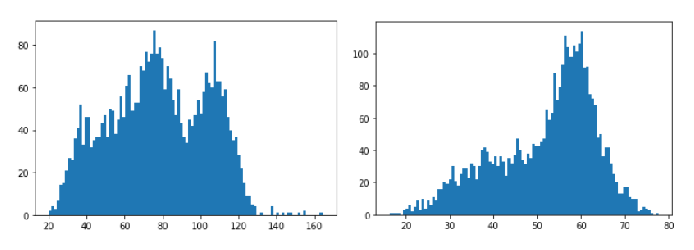
\includegraphics[width=12cm]{figures/fig01-combined.eps}
\caption{Distribution of brightness \textbf{(left)} and contrast \textbf{(right)} of training images.}\label{fig:1}
\end{figure}

\begin{figure}[H]
\centering
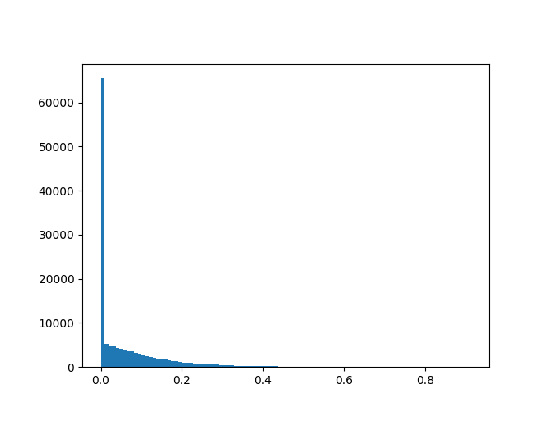
\includegraphics[width=6cm]{figures/fig02-iou.eps}
\caption{Distribution of IoU of labelled bounding boxes.}\label{fig:2}
\end{figure}


\begin{figure}[H]
\centering
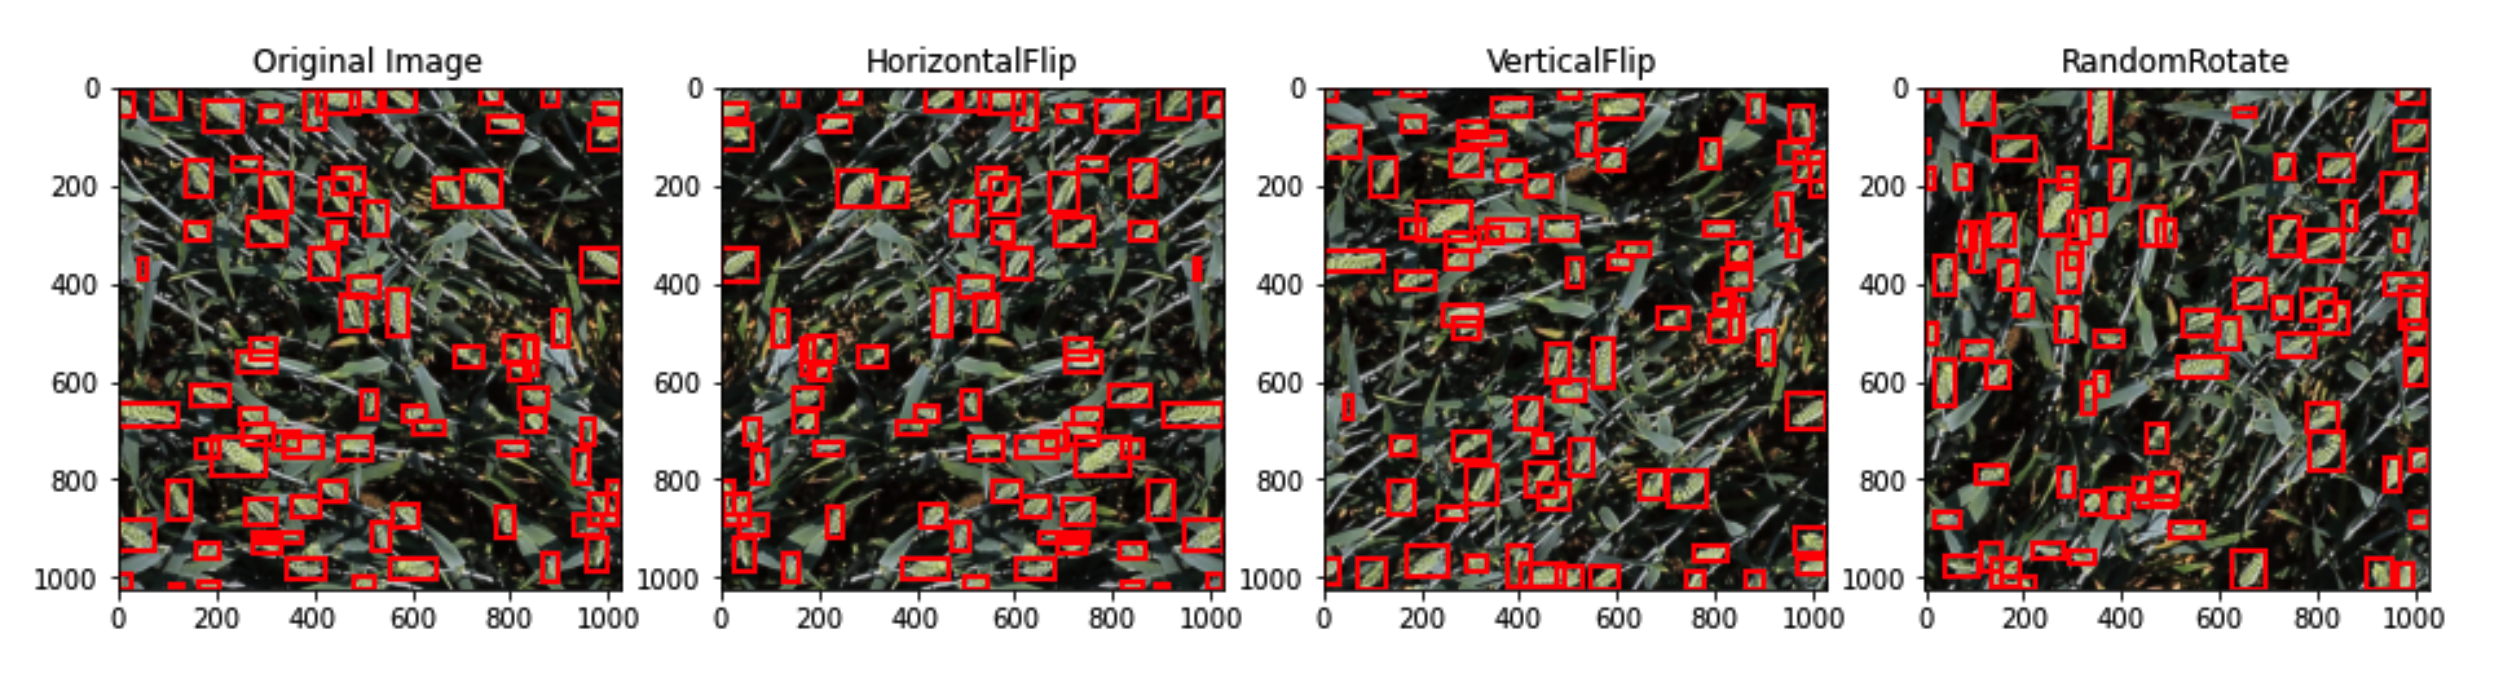
\includegraphics[width=15cm]{figures/fig03-horVerFlipRand.eps}
\caption{Image augmentation of HorizontalFlip, VerticalFlip, and RandomRotate}\label{fig:3}
\end{figure}

\begin{figure}[H]
\centering
\includegraphics[width=8cm]{figures/fig04-randBrightContrast.eps}
\caption{Image augmentation of RandomBrightnessContrast}\label{fig:4}
\end{figure}

\begin{figure}[H]
\centering
\includegraphics[width=8cm]{figures/fig05-HueSaturationValue.eps}
\caption{Image augmentation of HueSaturationValue}\label{fig:5}
\end{figure}

\begin{figure}[H]
\centering
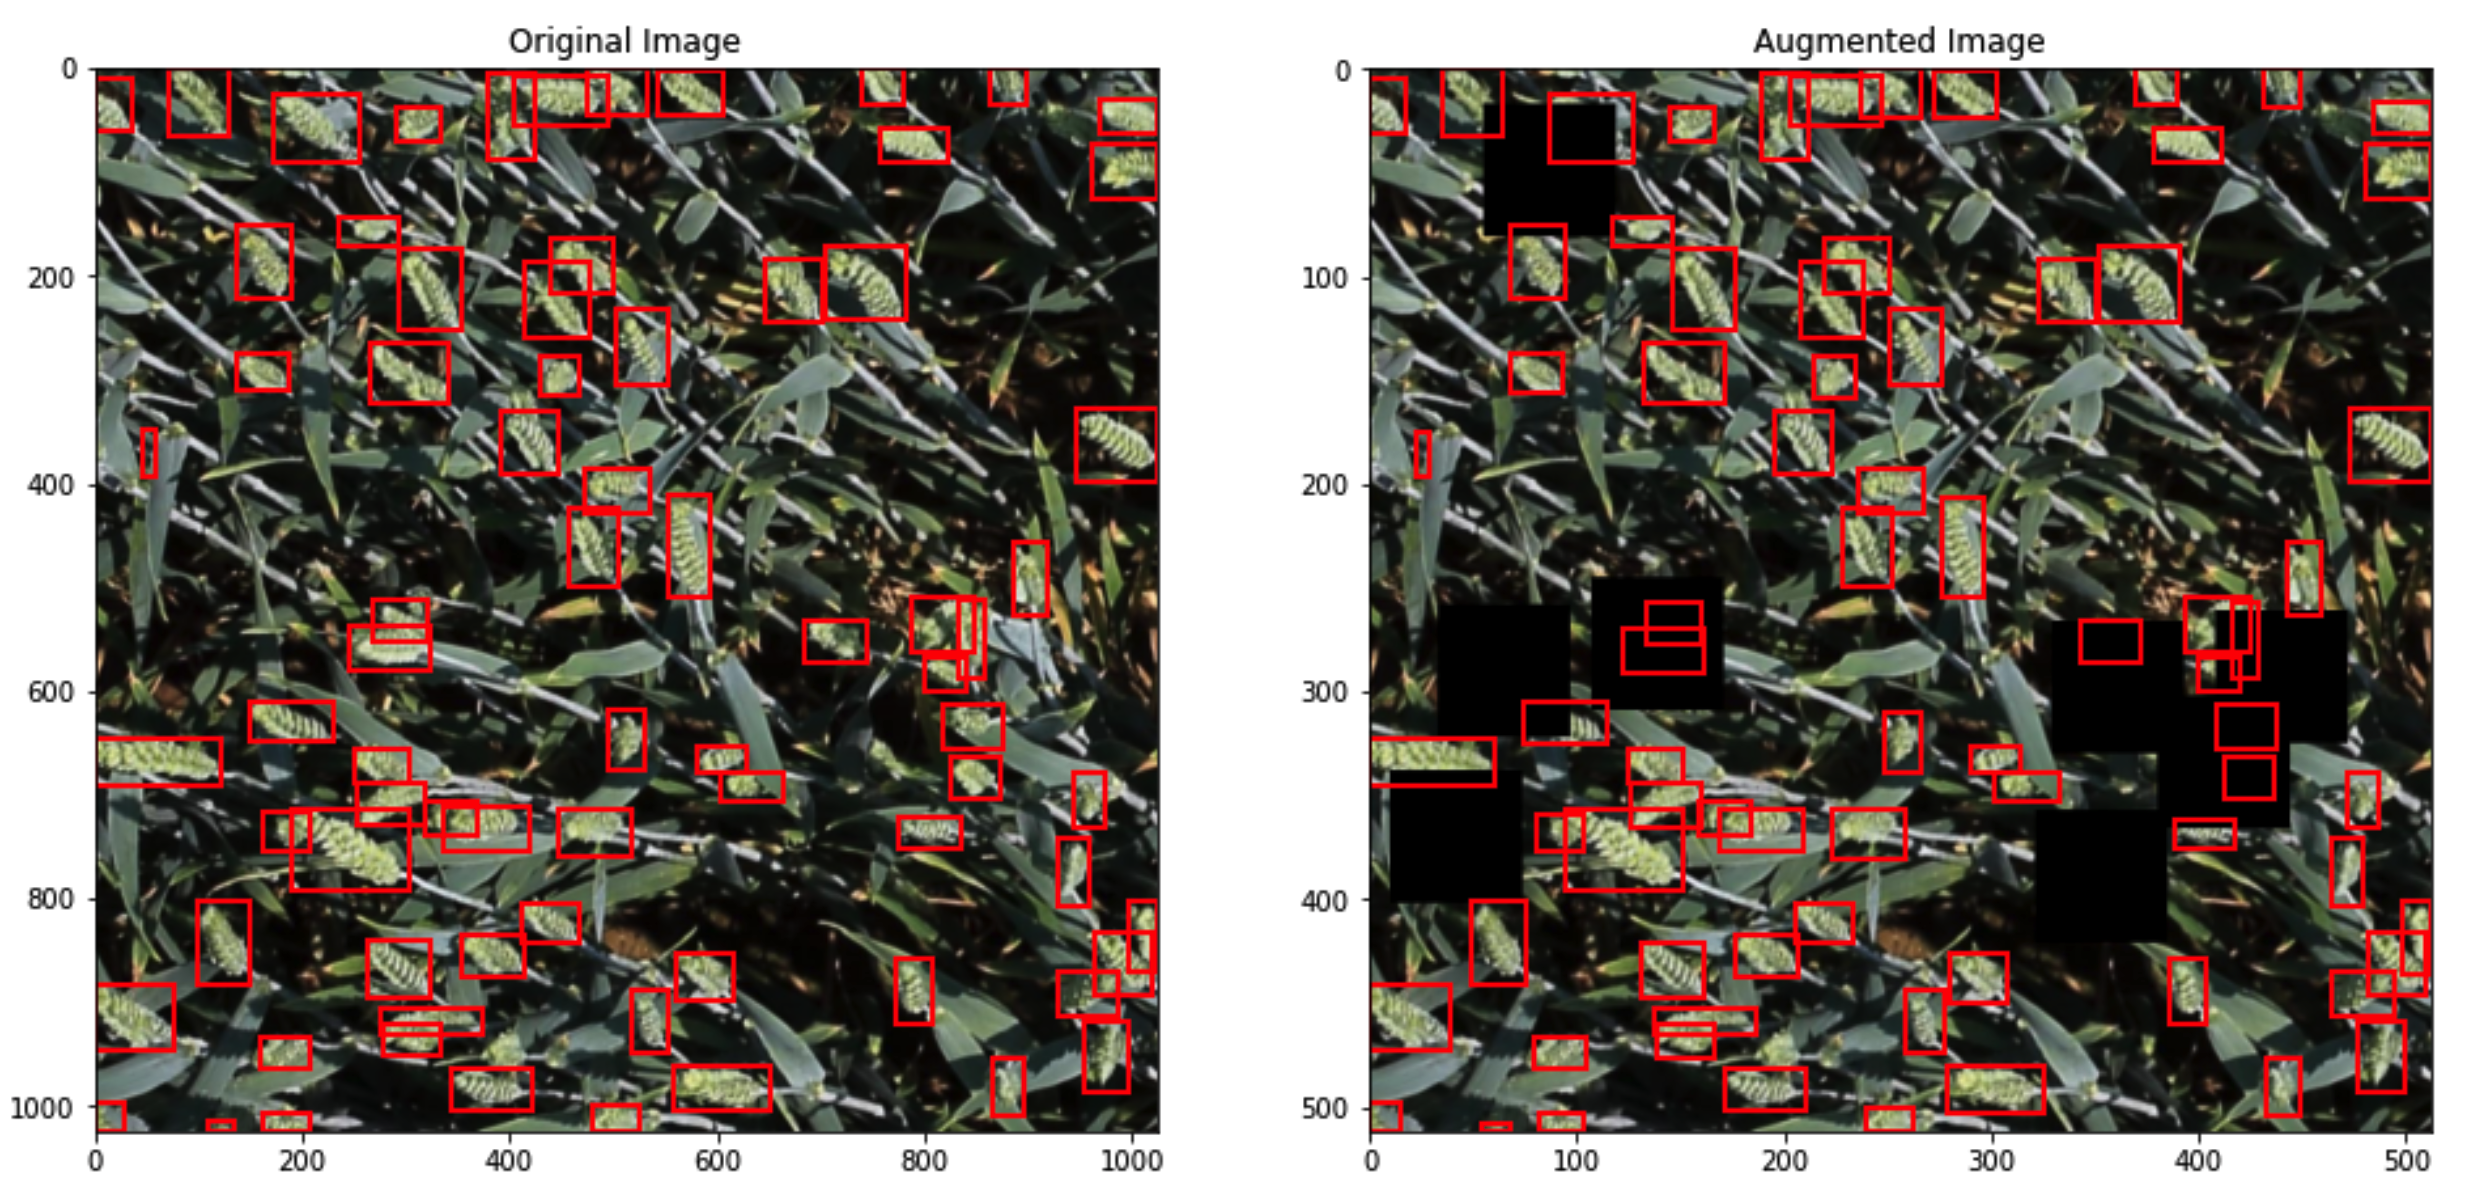
\includegraphics[width=8cm]{figures/fig06-coarseDropout.eps}
\caption{Image augmentation of CoarseDropout}\label{fig:6}
\end{figure}

\begin{figure}[H]
\centering
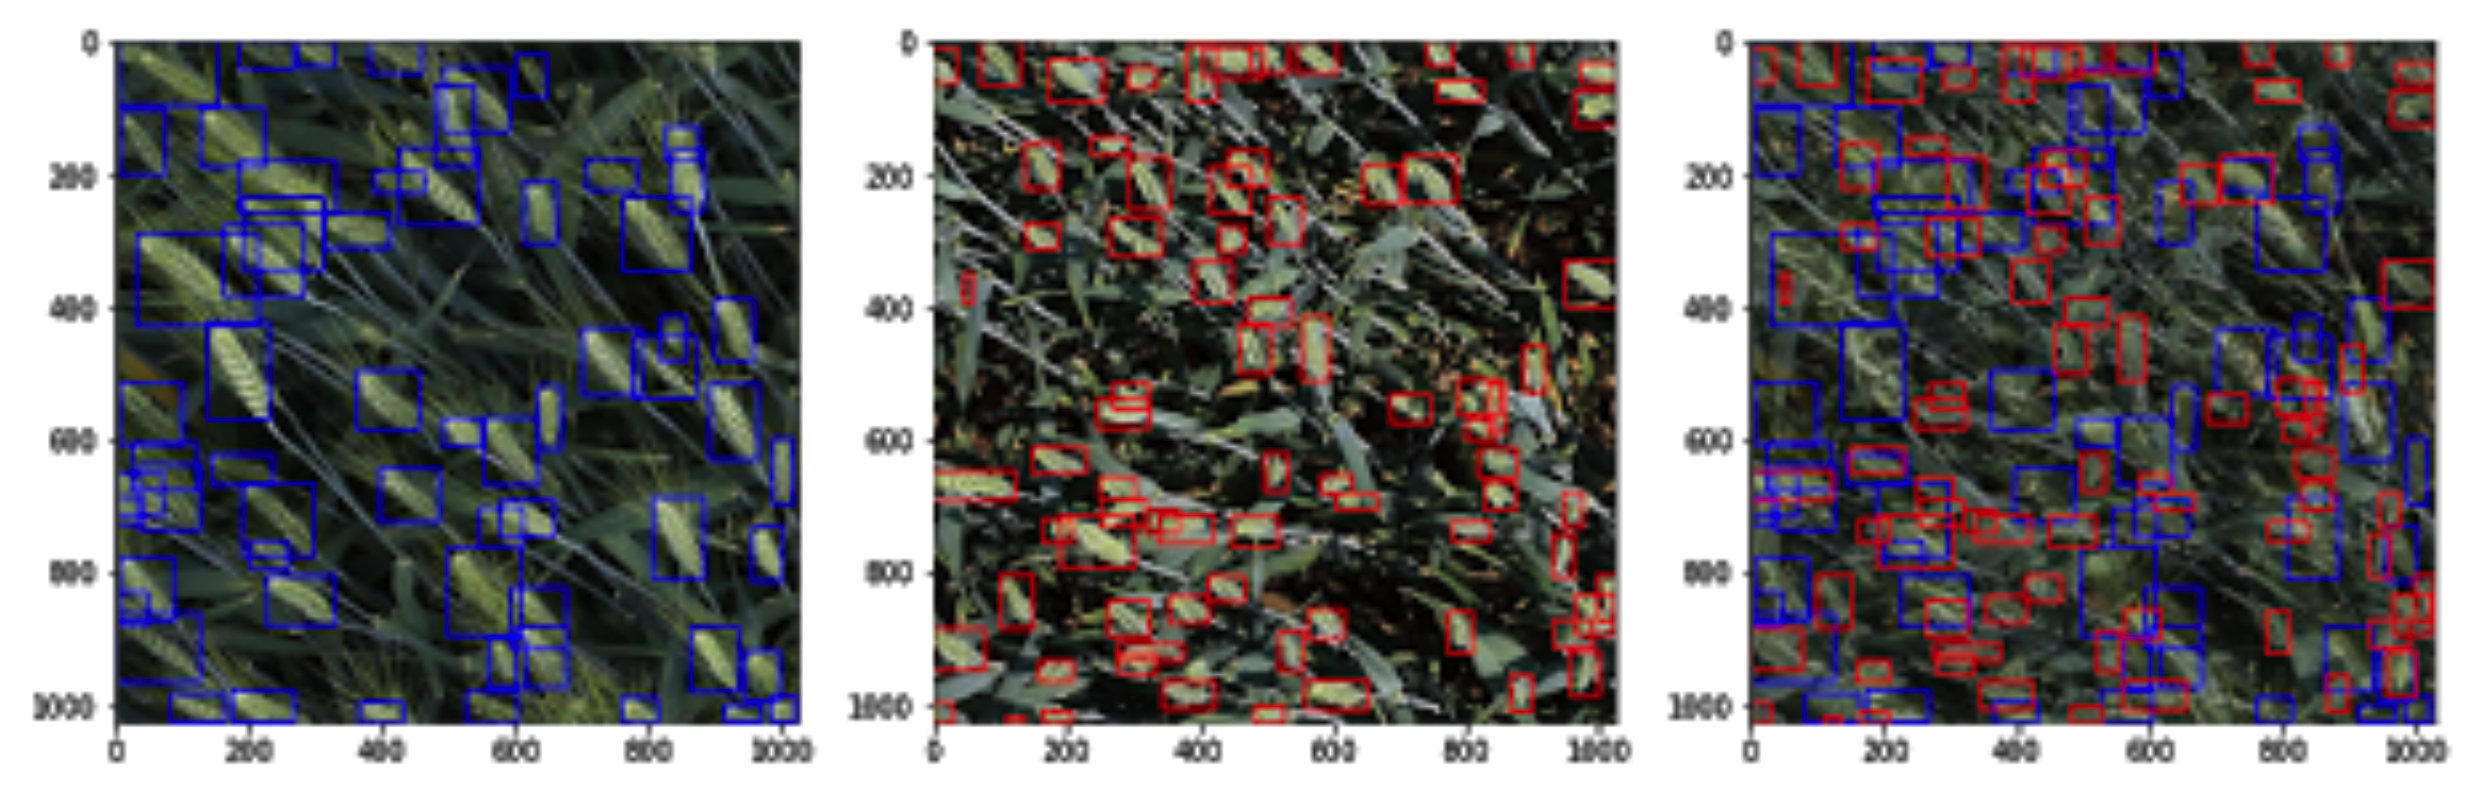
\includegraphics[width=8cm]{figures/fig07-mixup.eps}
\caption{Image augmentation of Mixup, using random selected image \textbf{(left)} and original image \textbf{(middle)} to generate the augmented image \textbf{(right)}.}\label{fig:7}
\end{figure}

\begin{figure}[H]
\centering
\includegraphics[width=8cm]{figures/fig08-PiecewiseAffine.eps}
\caption{Image augmentation of PiecewiseAffine}\label{fig:8}
\end{figure}

\begin{figure}[H]
\centering
\includegraphics[width=8cm]{figures/fig09-Blur.eps}
\caption{Image augmentation of Blur}\label{fig:9}
\end{figure}

\begin{figure}[H]
\centering
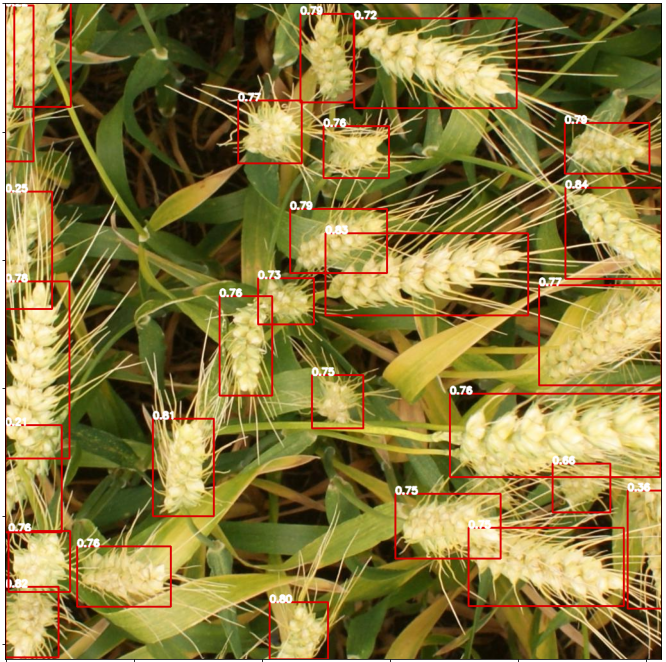
\includegraphics[width=6cm]{figures/fig10-yolo_sample.eps}
\caption{An example of output image using YOLO.}\label{fig:10}
\centering
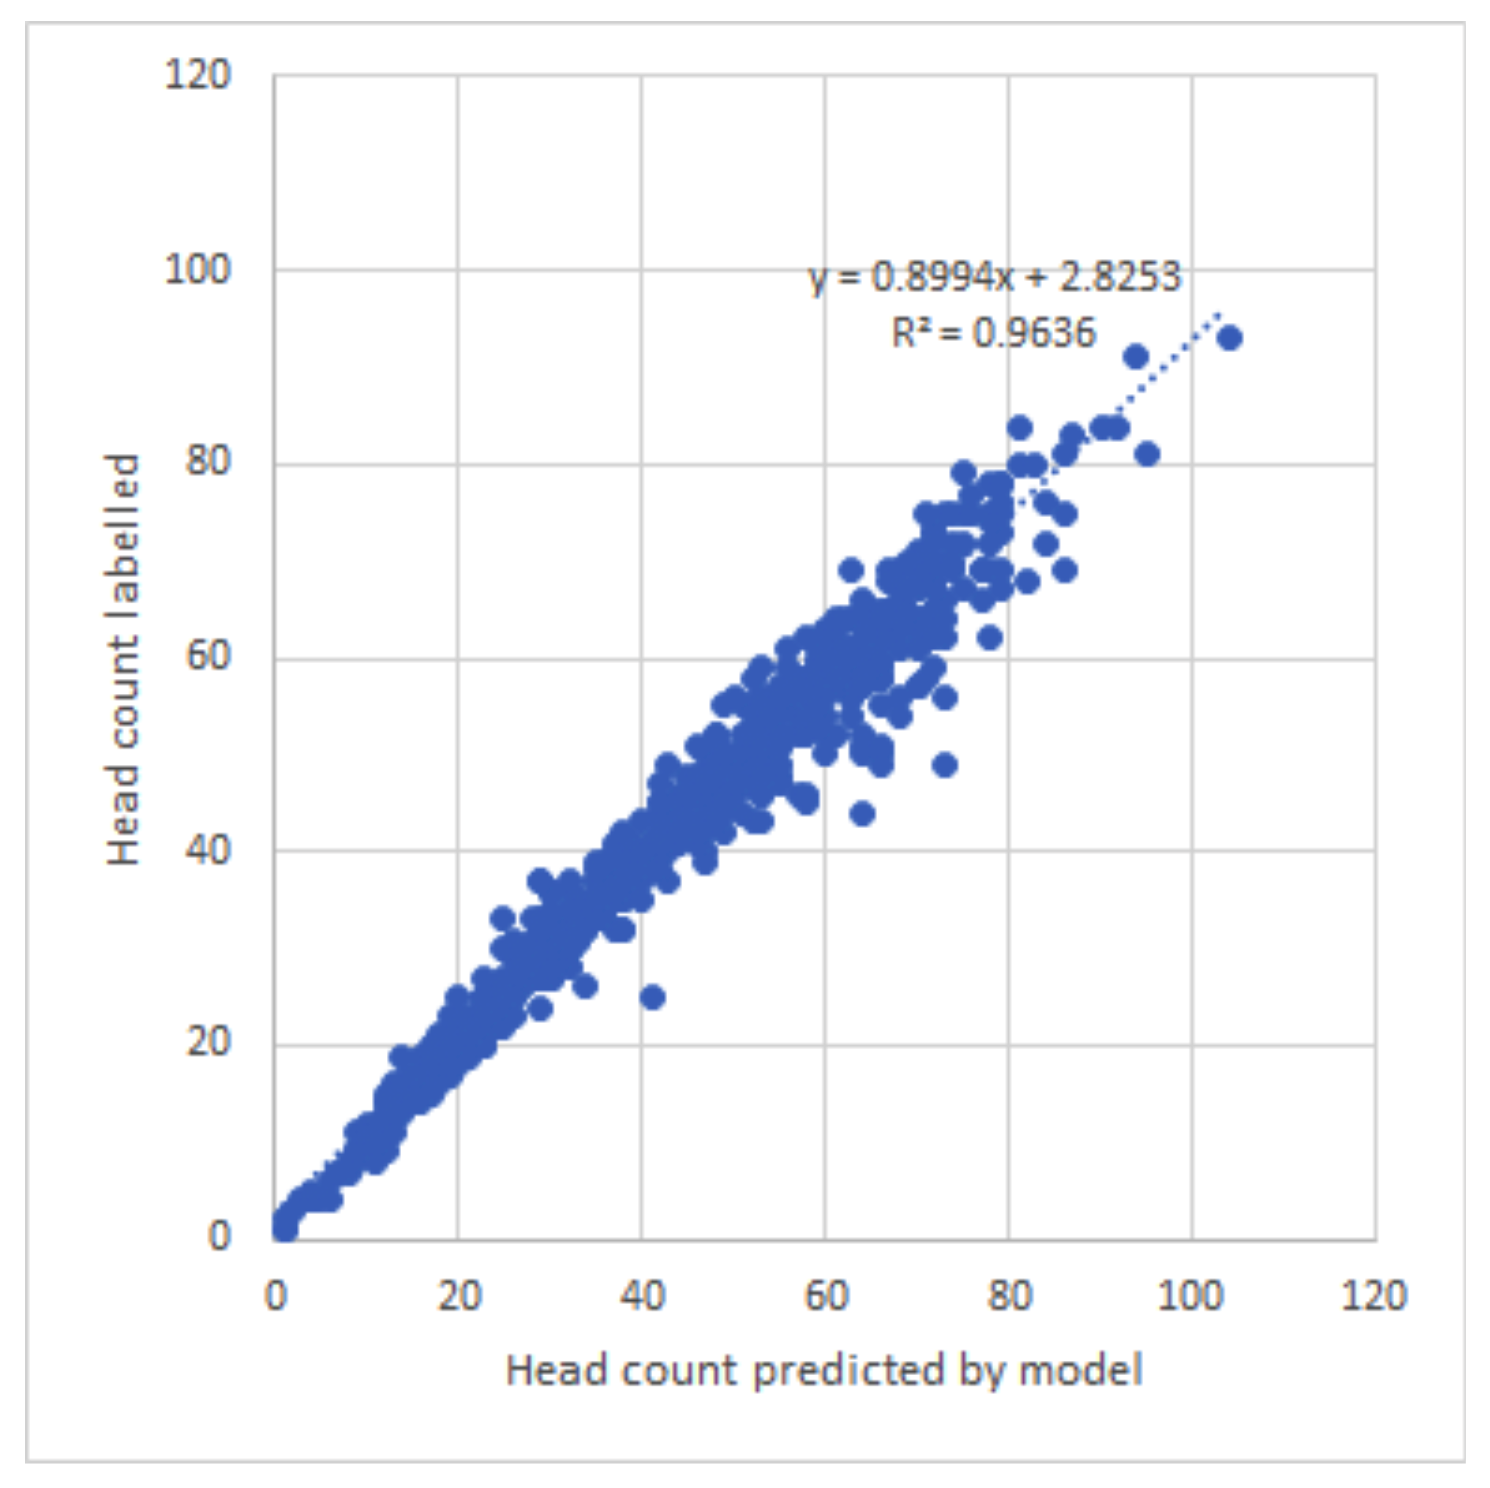
\includegraphics[width=6cm]{figures/fig11-YOLOcomp.eps}
\caption{Comparison between the number of head count in each image visually labelling and that detected using YOLO.}\label{fig:11}
\end{figure}

\begin{figure}[H]
\centering
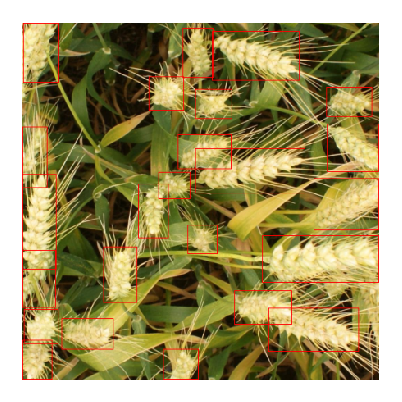
\includegraphics[width=6cm]{figures/fig12-eff_sample.eps}
\caption{An example of output image using EfficientDet.}\label{fig:12}
\centering
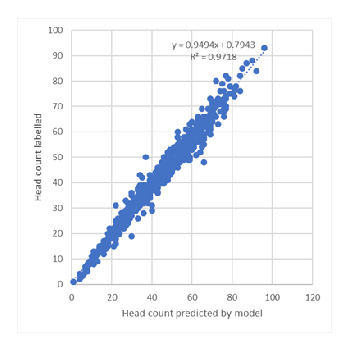
\includegraphics[width=6cm]{figures/fig13-val_eff.eps}
\caption{Comparison between the number of head count in each image visually labelling and that detected using EfficientDet.}\label{fig:13}
\end{figure}
\end{document}
